\documentclass[11pt,compress,t,notes=noshow, xcolor=table]{beamer}
\usepackage[]{graphicx}\usepackage[]{color}
% maxwidth is the original width if it is less than linewidth
% otherwise use linewidth (to make sure the graphics do not exceed the margin)
\makeatletter
\def\maxwidth{ %
  \ifdim\Gin@nat@width>\linewidth
    \linewidth
  \else
    \Gin@nat@width
  \fi
}
\makeatother

\newcommand{\citebutton}[2]{%
\beamergotobutton{\href{#2}{#1}}%
}

\newcommand{\blu}[1]{\textcolor{blue}{#1}}
\newcommand{\org}[1]{\textcolor{orange}{#1}}
\newcommand{\ques}{\textbf{\textcolor{red}{Question:  }}}
\newcommand{\questionssofar}{\begin{frame}\frametitle{Any questions?}\end{frame}}

\newcommand\warning{%
 \makebox[1.4em][c]{%
 \makebox[0pt][c]{\raisebox{.1em}{\scriptsize!}}%
 \makebox[0pt][c]{\color{red}\normalsize$\bigtriangleup$}}}%

\definecolor{fgcolor}{rgb}{0.345, 0.345, 0.345}
\newcommand{\hlnum}[1]{\textcolor[rgb]{0.686,0.059,0.569}{#1}}%
\newcommand{\hlstr}[1]{\textcolor[rgb]{0.192,0.494,0.8}{#1}}%
\newcommand{\hlcom}[1]{\textcolor[rgb]{0.678,0.584,0.686}{\textit{#1}}}%
\newcommand{\hlopt}[1]{\textcolor[rgb]{0,0,0}{#1}}%
\newcommand{\hlstd}[1]{\textcolor[rgb]{0.345,0.345,0.345}{#1}}%
\newcommand{\hlkwa}[1]{\textcolor[rgb]{0.161,0.373,0.58}{\textbf{#1}}}%
\newcommand{\hlkwb}[1]{\textcolor[rgb]{0.69,0.353,0.396}{#1}}%
\newcommand{\hlkwc}[1]{\textcolor[rgb]{0.333,0.667,0.333}{#1}}%
\newcommand{\hlkwd}[1]{\textcolor[rgb]{0.737,0.353,0.396}{\textbf{#1}}}%
\let\hlipl\hlkwb

\usepackage{framed}
\makeatletter
\newenvironment{kframe}{%
 \def\at@end@of@kframe{}%
 \ifinner\ifhmode%
  \def\at@end@of@kframe{\end{minipage}}%
  \begin{minipage}{\columnwidth}%
 \fi\fi%
 \def\FrameCommand##1{\hskip\@totalleftmargin \hskip-\fboxsep
 \colorbox{shadecolor}{##1}\hskip-\fboxsep
     % There is no \\@totalrightmargin, so:
     \hskip-\linewidth \hskip-\@totalleftmargin \hskip\columnwidth}%
 \MakeFramed {\advance\hsize-\width
   \@totalleftmargin\z@ \linewidth\hsize
   \@setminipage}}%
 {\par\unskip\endMakeFramed%
 \at@end@of@kframe}
\makeatother

\definecolor{shadecolor}{rgb}{.97, .97, .97}
\definecolor{messagecolor}{rgb}{0, 0, 0}
\definecolor{warningcolor}{rgb}{1, 0, 1}
\definecolor{errorcolor}{rgb}{1, 0, 0}
\newenvironment{knitrout}{}{} % an empty environment to be redefined in TeX

\usepackage{alltt}
\newcommand{\SweaveOpts}[1]{}  % do not interfere with LaTeX
\newcommand{\SweaveInput}[1]{} % because they are not real TeX commands
\newcommand{\Sexpr}[1]{}       % will only be parsed by R
\newcommand{\xmark}{\ding{55}}%


\usepackage[english]{babel}
\usepackage[utf8]{inputenc}

\usepackage{dsfont}
\usepackage{verbatim}
\usepackage{amsmath}
\usepackage{amsfonts}
\usepackage{amssymb}
\usepackage{bm}
\usepackage{csquotes}
\usepackage{multirow}
\usepackage{longtable}
\usepackage{booktabs}
\usepackage{enumerate}
\usepackage[absolute,overlay]{textpos}
\usepackage{psfrag}
\usepackage{algorithm}
\usepackage{algpseudocode}
\usepackage{eqnarray}
\usepackage{arydshln}
\usepackage{tabularx}
\usepackage{placeins}
\usepackage{tikz}
\usepackage{setspace}
\usepackage{colortbl}
\usepackage{mathtools}
\usepackage{wrapfig}
\usepackage{bm}
\usepackage{amsmath}
\usepackage{pifont}

\usetikzlibrary{shapes.multipart,shapes,arrows,automata,positioning,calc,chains,trees, shadows}
\tikzset{
  %Define standard arrow tip
  >=stealth',
  %Define style for boxes
  punkt/.style={
    rectangle,
    rounded corners,
    draw=black, very thick,
    text width=6.5em,
    minimum height=2em,
    text centered},
  % Define arrow style
  pil/.style={
    ->,
    thick,
    shorten <=2pt,
    shorten >=2pt,}
}

\tikzstyle{vec}=[draw, rectangle, fill = white, minimum width=5mm, minimum height=1cm, inner sep = 2pt]

\usepackage{subfig}

% Defines macros and environments
\usepackage{../../style/lmu-lecture}


\let\code=\texttt
\let\proglang=\textsf

\setkeys{Gin}{width=0.9\textwidth}

\setbeamertemplate{frametitle}{\expandafter\uppercase\expandafter\insertframetitle}

\usepackage{bbm}
% basic latex stuff
\newcommand{\pkg}[1]{{\fontseries{b}\selectfont #1}} %fontstyle for R packages
\newcommand{\lz}{\vspace{0.5cm}} %vertical space
\newcommand{\dlz}{\vspace{1cm}} %double vertical space
\newcommand{\oneliner}[1] % Oneliner for important statements
{\begin{block}{}\begin{center}\begin{Large}#1\end{Large}\end{center}\end{block}}


%new environments
\newenvironment{vbframe}  %frame with breaks and verbatim
{
 \begin{frame}[containsverbatim,allowframebreaks]
}
{
\end{frame}
}

\newenvironment{vframe}  %frame with verbatim without breaks (to avoid numbering one slided frames)
{
 \begin{frame}[containsverbatim]
}
{
\end{frame}
}

\newenvironment{blocki}[1]   % itemize block
{
 \begin{block}{#1}\begin{itemize}
}
{
\end{itemize}\end{block}
}

\newenvironment{fragileframe}[2]{  %fragile frame with framebreaks
\begin{frame}[allowframebreaks, fragile, environment = fragileframe]
\frametitle{#1}
#2}
{\end{frame}}


\newcommand{\myframe}[2]{  %short for frame with framebreaks
\begin{frame}[allowframebreaks]
\frametitle{#1}
#2
\end{frame}}

\newcommand{\remark}[1]{
  \textbf{Remark:} #1
}


\newenvironment{deleteframe}
{
\begingroup
\usebackgroundtemplate{
\includegraphics[width=\paperwidth,height=\paperheight]{../style/color/red.png}}
 \begin{frame}
}
{
\end{frame}
\endgroup
}
\newenvironment{simplifyframe}
{
\begingroup
\usebackgroundtemplate{
\includegraphics[width=\paperwidth,height=\paperheight]{../style/color/yellow.png}}
 \begin{frame}
}
{
\end{frame}
\endgroup
}\newenvironment{draftframe}
{
\begingroup
\usebackgroundtemplate{
\includegraphics[width=\paperwidth,height=\paperheight]{../style/color/green.jpg}}
 \begin{frame}
}
{
\end{frame}
\endgroup
}
% https://tex.stackexchange.com/a/261480: textcolor that works in mathmode
\makeatletter
\renewcommand*{\@textcolor}[3]{%
  \protect\leavevmode
  \begingroup
    \color#1{#2}#3%
  \endgroup
}
\makeatother





\input{../../latex-math/basic-math.tex}
\input{../../latex-math/basic-ml.tex}

%\newcommand{\titlefigure}{figure/gpt_sq.png}
\newcommand{\learninggoals}{
\item High level understanding of feed forward networks,
\item and the role and choices of activations}

\title{Deep Learning basics}
% \author{}
\institute{\href{https://slds-lmu.github.io/lecture_dl4nlp/}{slds-lmu.github.io/lecture\_dl4nlp}}
\date{}

\begin{document}
\lecturechapter{Deep Feedforward Networks}
\lecture{Deep Learning for NLP}

% ------------------------------------------------------------------------------

\begin{vbframe}{Deep Feedforward Networks}

\vfill

\begin{itemize}
\item Function approximation: find good mapping $\vec{\hat y} = f(\vec x; \vec \theta)$ (or more exactly $f(\vec x; \hat{\vec \theta})$,
     but we omit the hat in future).
\item \emph{Network}: Composition of functions $f^{(1)}, f^{(2)},f^{(3)}$ with multi-dimensional input and output
\item Each $f^{(i)}$ represents one \emph{layer}
$f(\vec x) = f^{(1)}( f^{(2)}(f^{(3)}(\vec x))))$

\item \emph{Feedforward}: 

\begin{itemize}
\item Input $\rightarrow$ intermediate representation $\rightarrow$ output
\item No feedback connections
\item Cf. \emph{recurrent} networks
\end{itemize}
\end{itemize}
\begin{center}
%\includegraphics[width = 0.5\textwidth]{./}
\end{center}

\vfill

\end{vbframe}


% ------------------------------------------------------------------------------

\begin{vbframe}{Deep Feedforward Networks: Training}

\vfill

\begin{itemize}
\item Loss function defined on output layer, e.g. $(y - f(\vec x; \vec \theta))^2$
\item Quality criterion on other layers not directly defined.
\item Training algorithm must decide how to use those layers most effectively (w.r.t. loss on output layer)
\item Non-output layers can be viewed as providing a feature function $\phi(\vec x)$ of the input, that is to be learned.
\end{itemize}
\begin{center}
%\includegraphics[width = 0.5\textwidth]{./}
\end{center}

\vfill

\end{vbframe}


% ------------------------------------------------------------------------------

\begin{vbframe}{\emph{``Neural''} Networks}

\vfill

\begin{itemize}
\item Inspired by biological neurons (nerve cells)
\item Neurons are connected to each other, and receive and send electrical pulses.
\item \emph{``If the [input] voltage changes by a large enough amount, an all-or-none electrochemical pulse called an action potential is generated, which travels rapidly along the cell's axon, and activates synaptic connections with other cells when it arrives.''} (Wikipedia)
\end{itemize}

\begin{center}
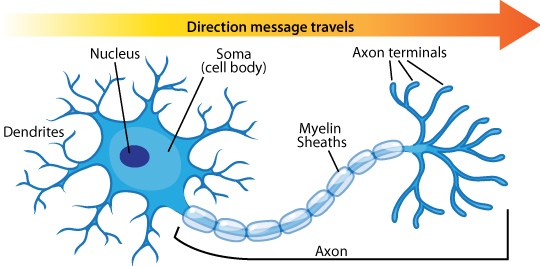
\includegraphics[width = 0.5\textwidth]{./figure/neuron_anatomy}
\end{center}


\vfill

\end{vbframe}


% ------------------------------------------------------------------------------

\begin{vbframe}{Activation Functions with Non-Linearities}

\vfill

\begin{itemize}
\item Linear Functions are limited in what they can express.
\item Famous example: XOR
\item Simple layered non-linear functions can represent XOR.
\end{itemize}
\begin{center}
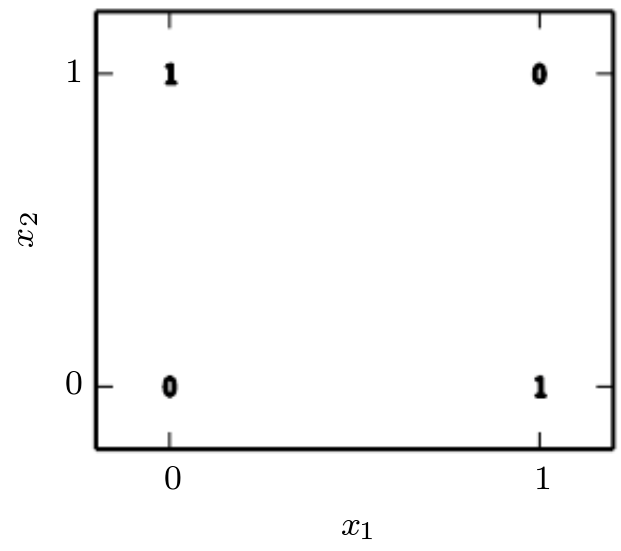
\includegraphics[width = 0.5\textwidth]{./figure/xor}
\end{center}

\vfill

\end{vbframe}


% ------------------------------------------------------------------------------

\begin{vbframe}{Design Choices for Output Units}

\vfill

\begin{itemize}
\item Can typically be interpreted as probabilities.
\begin{itemize}
\item Logistic sigmoid
\item Softmax
\item mean and variance of a Gaussian, ...
\end{itemize}
\item Trained with negative log-likelihood.
\end{itemize}
\begin{center}
%\includegraphics[width = 0.5\textwidth]{./}
\end{center}

\vfill

\end{vbframe}


% ------------------------------------------------------------------------------

\begin{vbframe}{Softmax}

\vfill

\begin{itemize}
\item Logistic sigmoid \\
\begin{itemize}
\item Vector $\vec y$ of binary outcomes, with no contraints on how many can be 1.
\item Bernoulli distribution.
\end{itemize}
\item Softmax
\begin{itemize}
\item Exactly one element of $\vec y$ is 1.
\item Multinoulli (categorical) distribution.
$$p(Y = i| \vec{\phi}(\vec x))$$
$$\sum_i p(Y = i| \vec{\phi}(\vec x)) = 1$$
$$softmax(\vec z)_i = \frac{exp(z_i)}{\sum_j exp(z_j)}$$
\end{itemize}
\end{itemize}
\begin{center}
%\includegraphics[width = 0.5\textwidth]{./}
\end{center}

\vfill

\end{vbframe}


% ------------------------------------------------------------------------------

\begin{vbframe}{Parametrizing a Gaussian Distribution}

\vfill

\begin{itemize}
\item Use final layer to predict parameters of Gaussian mixture model.
\item Weight of mixture component: softmax.
\item Means: no non-linearity.
\item Precisions ($\frac{1}{\sigma^2}$) need to be positive: softplus
$$softplus(z) = ln(1+exp(z))$$
\end{itemize}
\begin{center}
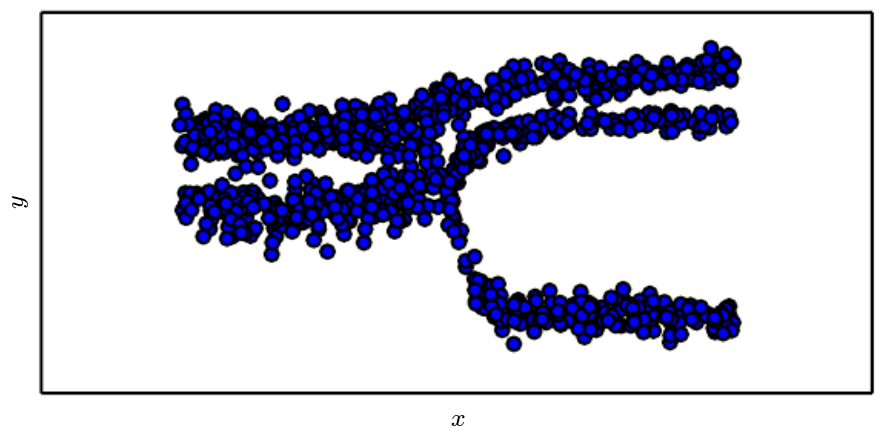
\includegraphics[width = 0.7\textwidth]{./figure/gaussian_mixture_samples}
\end{center}

\vfill

\end{vbframe}


% ------------------------------------------------------------------------------

\begin{vbframe}{Design Choices for Hidden Units}

\vfill

\begin{itemize}
\item Rectified Linear Unit:
$$relu(z) = max(0,z)$$
$$z = \vec x^T\vec w + b$$
\begin{center}
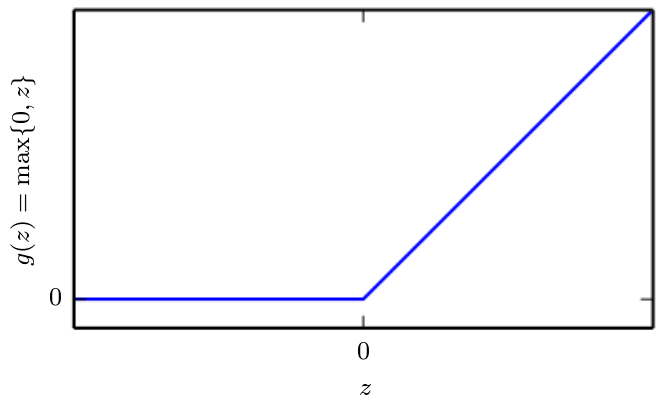
\includegraphics[width = 0.5\textwidth]{./figure/relu}
\end{center}
\item Consistent gradient of 1 when unit is \emph{active} (i.e. if there is an error to propagate).
\item Default choice for hidden units.
\end{itemize}

\vfill

\end{vbframe}


% ------------------------------------------------------------------------------

\begin{vbframe}{A Simple ReLU Network to Solve XOR}

\vfill

$$f(\vec x; \vec W, \vec c, \vec w) = \vec w^T max(0, \vec W^T\vec x + \vec c)$$

\[\vec W = 
\begin{bmatrix}
 1 & 1 \\
 1 & 1
\end{bmatrix} 
\]

\[\vec c = 
\begin{bmatrix}
 0 \\
 -1
\end{bmatrix} 
\]

\[\vec w = 
\begin{bmatrix}
 1 \\
 -2
\end{bmatrix} 
\]

\vfill

\end{vbframe}


% ------------------------------------------------------------------------------

\begin{vbframe}{Other Choices for Hidden Units}

\vfill

\begin{itemize}
\item A good activation function aids learning, and provides large gradients.
\item Sigmoidal functions (logistic sigmoid)
\begin{itemize}
 \item have only a small region before they flatten out in either direction.
 \item Practice shows that this seems to be ok in conjunction with Log-loss objective.
 \item But they don't work as well as hidden units.
 \item ReLU are better alternative since gradient stays constant.
\end{itemize}
\item Other hidden unit functions:
\begin{itemize}
 \item maxout: take maximum of several values in previous layer.
 \item purely linear: can serve as low-rank approximation.
\end{itemize}
\end{itemize}
\begin{center}
%\includegraphics[width = 0.5\textwidth]{./}
\end{center}

\vfill

\end{vbframe}


\endlecture
\end{document}
